\chapter{Introduzione a PYNQ board}

PYNQ è un progetto open-source gestito da Xilinx che porta le funzionalità di una FPGA a linguaggi ad alto livello.

\begin{figure}[H]
    \centering
    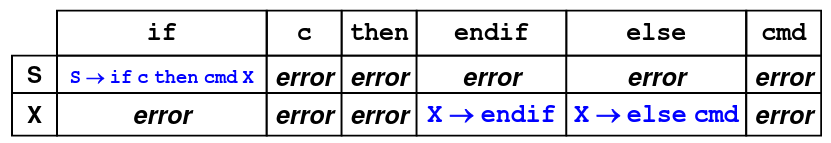
\includegraphics[width=0.7\textwidth]{/home/riccardoob/appunti/sistemi_digitali/images/16.png}
\end{figure}

La PYNQ board monta un processore dual-core ARM Cortex-A9, chiamato \textbf{Processing System} (PS), e una FPGA (\textbf{Porgrammable Logic}, PL).

Il PS può richiedere l'esecuzione di alcune funzione al PL, utilizzando chiamate a librerie hardware specifiche, chiamate \textbf{overlays}.
\begin{figure}[H]
    \centering
    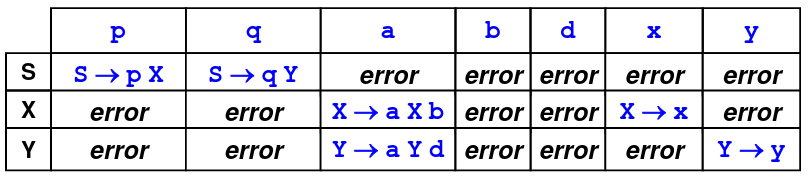
\includegraphics[width=0.7\textwidth]{/home/riccardoob/appunti/sistemi_digitali/images/17.png}
\end{figure}

Possono essere caricate alla FPGA dinamicamente e chiamate quando necessario, in questo gli overlay sono similari a librerie software.

É resa disponibile una interfaccia Python, utile per controllare overlays caricati nel PL da codice Python eseguito sul PS.

\subsubsection{Primi passi}
La board è provvista di una scheda SD con una versione di PYNQ, una distro linux custom.

Può essere collegata direttamente a un PC, e una volta accesa e collegata a un router, è possibile accedere a un web server, solitamente all'indirizzo \url{http://pynq:9090} (se connesso tramite ethernet) o a \url{http://192.168.2.99:9090}.

\section{Overlay}
Gli overlay permettono di utilizziare IP di basso livello tramite Python. Un overlay carica un \textbf{bitstream} per permettere l'accesso alle sue funzionalità: per questo si utilizzano oggetti \textbf{driver}.

\subsubsection{Esempio}
Ad esempio, si considera una semplice funzione HLS che restituisce la somma di due int a 32 bit.
\begin{minted}[bgcolor=lightgray,framesep=2mm,baselinestretch=1.2,fontsize=\footnotesize]{c}
void add(int a, int b, int &c) {
    #pragma HLS INTERFACE ap_ctrl_none port=return
    #pragma HLS INTERFACE s_axilite port=a
    #pragma HLS INTERFACE s_axilite port=b
    #pragma HLS INTERFACE s_axilite port=c

    c = a + b;
}
\end{minted}
Dopo aver progettato l'IP è possibile importarla in python creando un overlay tramite il pacchetto \texttt{pynq}, usato per caricare l'IP dal bitstream:
\begin{minted}[bgcolor=lightgray,framesep=2mm,baselinestretch=1.2,fontsize=\footnotesize]{python}
from pynq import Overlay

overlay = Overlay('/home/cilinx/tutorial_1.bit')
add_ip = overlay.scalar_add
help(add_ip)
\end{minted}
Con la funzione help è possibile ottenere informazione sull'oggetto IP estratto dall'overlay.

\begin{multicols}{2}
    L'IP core è caricato come oggetto base \texttt{DefaultIP}, un driver che espone API di \texttt{read} e \texttt{write}.
    
    Per l'esempio dell'add, secondo la documentazione, è necessario scrivere i due parametri della funzione agli offset \texttt{0x10} e \texttt{0x18} e leggere il risultato da \texttt{0x20}.
    \begin{minted}[bgcolor=lightgray,framesep=2mm,baselinestretch=1.2,fontsize=\footnotesize]{python}
add_ip.write(0x10, 4)
add_ip.write(0x18, 5)
add_ip.read(0x20) # 9
    \end{minted}
    \columnbreak
    \begin{multicolfigure}
        \centering
        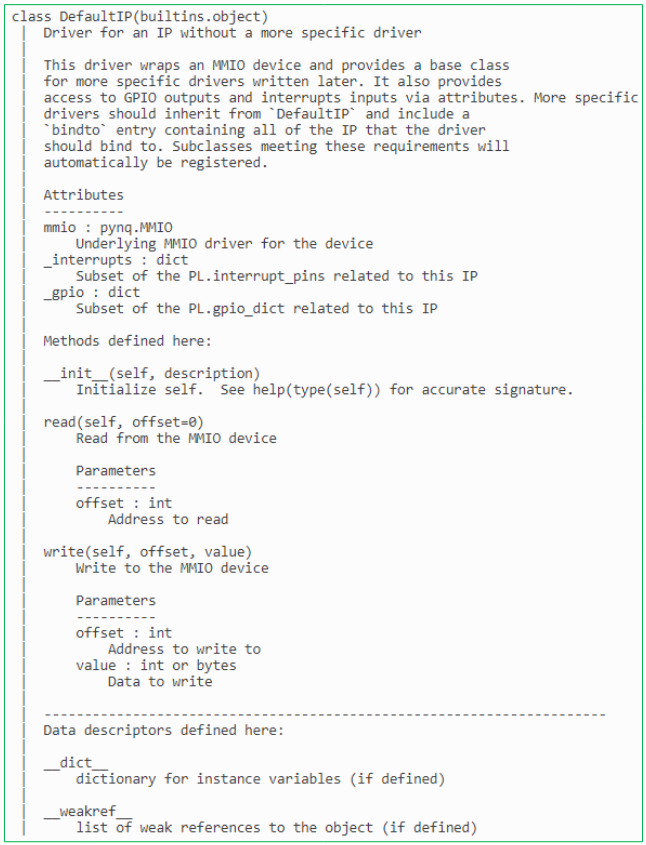
\includegraphics[width=\textwidth]{/home/riccardoob/appunti/sistemi_digitali/images/18.png}
    \end{multicolfigure}
\end{multicols}

Il driver di defualt non è user-friendly, una soluzione migliore è quella di creare una classe che estende il driver defualt e espone un metodo \texttt{add(a, b)} che implementa le operazioni necessarie.

\begin{minted}[bgcolor=lightgray,framesep=2mm,baselinestretch=1.2,fontsize=\footnotesize]{python}
class AddDriver(DefaultIP):
    def __init__(self, description):
        super().__init__(description=description)

    bindto = ['xilinx.com:hls:add:1.0']

    def add (self, a, b):
        self.write(0x10, a)
        self.write(0x18, b)
        return self.read(0x20)
\end{minted}

Ora è possibile accedere l'IP usando una singola \texttt{add} API, resa disponibile dal driver custom.

\subsubsection{Driver inclusi}
\begin{itemize}
    \item AXI GPIO
    \item AXI DMA
    \item AXI VDMA
    \item AXI Interrupt Controller
    \item Pynq-Z1 Audio IP
    \item Pynq-Z1 HDMI IP
    \item Color convert IP
    \item Pixel format conversion
    \item HDMI input and output frontends
    \item Pynq Microblaze program loading
    \item ...
\end{itemize}

\section{PYNQ Hello LED}
Gli overlay base che controllano le periferiche presenti sulla PYNQ, disponibili caricando il \texttt{BaseOverlay} da \texttt{pynq.overlay.base}:
\begin{minted}[bgcolor=lightgray,framesep=2mm,baselinestretch=1.2,fontsize=\footnotesize]{python}
import time
from pynq.overlays.base import BaseOverlay
base = BaseOverlay('base.bit')
\end{minted}

É possibile, ad esempio, accedere a singoli LED e accenderli/spegnerli.
\begin{minted}[bgcolor=lightgray,framesep=2mm,baselinestretch=1.2,fontsize=\footnotesize]{python}
led0 = base.leds[0]
led1 = base.leds[1]
led2 = base.leds[2]
led3 = base.leds[3]

led0.on()
led0.off()
\end{minted}

É anche possibile utilizzare switch per interagire con i led, per prima cosa si ottengono i LED, switch e tasti disponibili.
\begin{minted}[bgcolor=lightgray,framesep=2mm,baselinestretch=1.2,fontsize=\footnotesize]{python}
MAX_LED = 4
MAX_SWITCHES = 2
MAX_BUTTONS = 4

leds = [0] * MAX_LEDS
switches = [0] * MAX_SWITCHES
buttons = [0] * MAX_BUTTONS

for i in range(MAX_LEDS):
    leds[i] = base.leds[i]
for i in range(MAX_SWITCHES):
    leds[i] = base.switches[i]
for i in range(MAX_BUTTONS):
    leds[i] = base.buttons[i]
\end{minted}
\textbf{INSERIRE25-26}

\section{HDMI Stream}
La board mette a disposizione driver per gestire le porte HDMI:
\begin{minted}[bgcolor=lightgray,framesep=2mm,baselinestretch=1.2,fontsize=\footnotesize]{python}
from pynq.overlays.base import BaseOverlay
from pynq.lib.video import *

base = BaseOverlay('base.bit')
hdmi_in = base.video.hdmi_in
hdmi_out = base.video.hdmi_out

# HDMI handlers configuration
hdmi_in.configure()
hdmi_out.configure(hdmi_in.mode)

hdmi_in.start()
hdmi_out.start()
\end{minted}

Come primo passo, è possibile semplicemente replicare l'input stream sull'HDMI output utilizzando \texttt{hdmi\_in.tie(hdmi\_out)}.

Con lo stesso risultato, è possibile inoltrare frame per frame da input ad ouput, utilizzando i metodi \texttt{readframe} e \texttt{writeframe}.
\begin{minted}[bgcolor=lightgray,framesep=2mm,baselinestretch=1.2,fontsize=\footnotesize]{python}
import time

numframes = 600
start = time.time()

for \_ in range(numframes):
    f = hdmi_in.readframe()
    hdmi_out.writeframe(f)

end = time.time()
print("Frames per second: " + str(numframes / (end - start)))
\end{minted}

Questo approccio permette di elaborare singoli frame prima di inviarli all'output.
\vspace{-0.8cm}
\begin{minted}[bgcolor=lightgray,framesep=2mm,baselinestretch=1.2,fontsize=\footnotesize]{python}
import cv2
import numpy as np

numframes = 10
grayscale = np.ndarray(shape=(hdmi_in.mode.height, hdmi_in.mode.width),
                       dtype=np.uint8)
result = np.ndarray(shape=(hdmi_in.mode.height, hdmi_in.mode.width),
                    dtype=np.uint8)

start = time.time()

for _ in range(numframes):
    inframe = hdmi_in.readframe()
    cv2.cvtcolor(inframe, cv2.COLOR_BGR2GRAY, dst=grayscale)
    inframe.freebuffer()
    cv2.Laplacian(grayscale, cv2.CV_8U, dst=result)

    outframe = hdmi_out.newframe()
    cv2.cvtcolor(result, cv2.COLOR_GRAY2BGR, dst = outframe)
    hdmi_out.writeframe(outframe)

end = time.time()
print("Frames per second: " + str(numframes / (end - start)))
\end{minted}

Ricordare di chiudere gli stream
\begin{minted}[bgcolor=lightgray,framesep=2mm,baselinestretch=1.2,fontsize=\footnotesize]{python}
hdmi_out.close()
hdmi_in.close()
\end{minted}

\section{Filtraggio accellerato HW}
Si estende l'esempio precedente con elaborazione di immagini hardware accelerated.

Si utilizza il modulo \texttt{overlay} per caricare un bitstream custom contenente il modulo di filtraggio 2D.

Si importa anche il modulo \texttt{xlnk}, un \textbf{memory manager}





































